\section{Apéndice 2. XML Schema descriptivo del archivo de exportación del contenido del fichero DWG.}

%\lstinputlisting[language=XML,breaklines=true]{xml/XSD_v3.xsd}
\begin{figure}[H]
\begin{center}
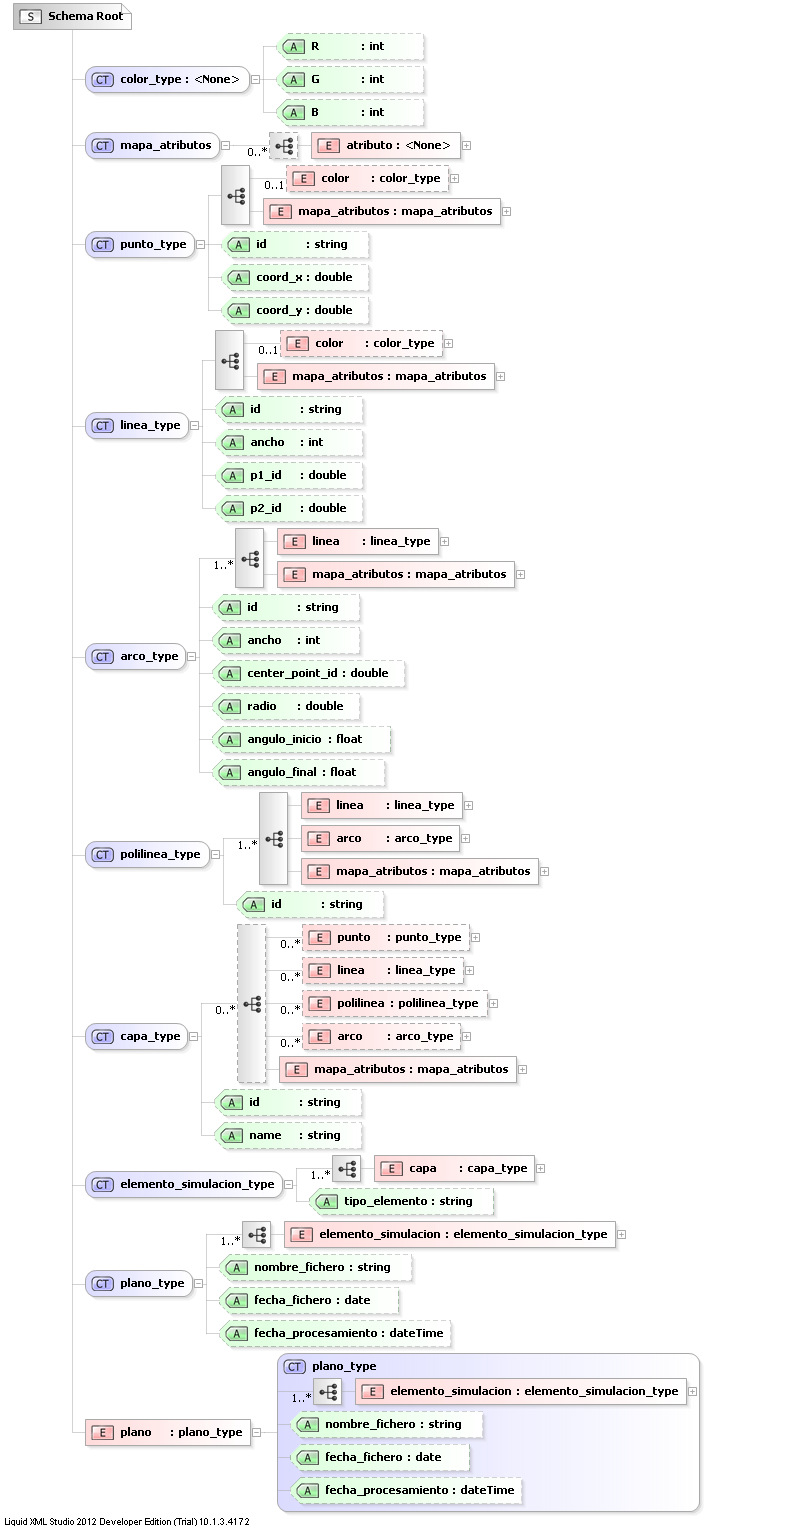
\includegraphics[height=\textheight]{imgs/XSD_v3}
\caption{XML Schema del fichero de salida del proceso de exportación.}
\end{center}
\end{figure}

El fichero de intercambio comienza con un elemento raíz \emph{plano}. Este elemento raíz esta caracterizado por los atributos:

\begin{itemize}

\item{nombre\_fichero: identifica el nombre del fichero DWG original cuyo contenido esta representado en el fichero XML.}

\item{fecha\_fichero: fecha de creación del fichero DWG original cuyo contenido esta representado en el fichero XML.}

\item{fecha\_procesamiento: marca de tiempo reflejando el momento en el que el fichero DWG original fue procesado y se genero el fichero XML.}

\end{itemize}

Del elemento raíz \emph{plano} dependen otros elementos del tipo \emph{elemento\_simulación}. Estos elementos representan los diferentes objetos identificados en el plano y que corresponden con diferentes objetos de las infraestructuras aéreas, como son pistas, taxiway-centerlines, etc. Los elementos de simulación se caracterizan por Esos elementos serán creados por los procesos de aprendizaje y reconocimiento de formas. El proceso de extracción sólo genera un tipo de elemento y es el <<elemento\_original\_mapa>>. Cada tipo de elemento esta caracterizado por los atributos:

\begin{itemize}

\item{tipo\_elemento: literal de texto que describe el tipo de elemento.}

\end{itemize}

Dentro de cada tipo\_elemento se anidan diferentes elementos \emph{capa}. Los elementos capas se caracterizan por los atributos:

\begin{itemize}

\item{id: identificador único de la capa.}
\item{nombre: nombre otorgado por el autor del dibujo a la capa.}

\end{itemize}

En cada elemento capa se anidan un número variable de diferentes elementos que representan los elementos gráficos exportados del fichero DWG. Cada elemento presenta los atributos ya descritos en las clases correspondientes del paquete dwgElementos. En concreto se pueden anidar los elementos:


\begin{itemize}

\item{Punto.}
\item{Línea.}
\item{Arco.}
\item{Polilínea.}

\end{itemize}

Otro elemento que puede encontrarse anidado dentro de los elementos punto y línea es el elemento \emph{color} que contiene en sus atributos los valores de un código de color RGB. 

Finalmente, existe otro elemento que puede encontrarse anidado dentro de los elementos punto, linea, polilínea y arco, el elemento \emph{mapa\_atributos}. Este elemento representa una colección de pares atributo-valor que permite asociar a cada elemento un número variable de propiedades con sus respectivos valores sin necesidad de predeterminar a priori las mismas. Este elemento es importante para dar cobertura a las posibles propiedades personalizadas creadas por un usuario dentro de AutoCAD.